\subsection{Specim IQ}

\subsubsection{Preview}

A spectral image by SpecimIQ was loaded by the Python script shown in Code \ref{code:load-envi} and converted to RGB preview by Code \ref{code:rgb-preview}. The gray scale preview and RGB preview are shown in Figure \ref{fig:specim-preview}.

Gray preview of the image was created by the following code:

\begin{lstlisting}[language=python, caption=Show gray scale preview, label={code:show-gray-preview}]
from pathlib import Path

path = Path('ASI course 2024/group3/Session1/Specim scanner/Color_checker_8_binning/capture/solutions_scan_0110')
spectral_image, envi_header = load_spectral_image(path)
plt.imshow(spectral_image[:, :, 100], cmap="gray")
\end{lstlisting}

RGB preview of the image was created by the following code:

\begin{lstlisting}[language=python, caption=Show RGB preview, label={code:show-rgb-preview}]
rgb_view = reconstruct_rgb_envi(spectral_image, envi_header)
plt.imshow(rgb_view)
\end{lstlisting}

Functions used in Code \ref{code:show-gray-preview} and Code \ref{code:show-rgb-preview} are defined in Code \ref{code:load-envi} and Code \ref{code:rgb-preview}.

\begin{figure}[H] %
  \centering
  \subfloat[Gray scale preview]{%
    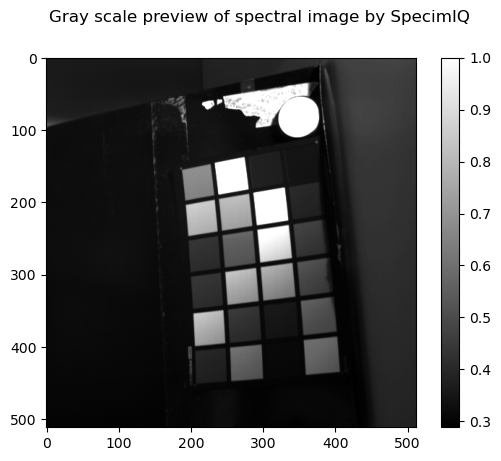
\includegraphics[width=0.45\textwidth]{fig-task1/specimIQ-gray.png}
  }
  \hspace{0.1cm}
  \subfloat[RGB preview]{%
    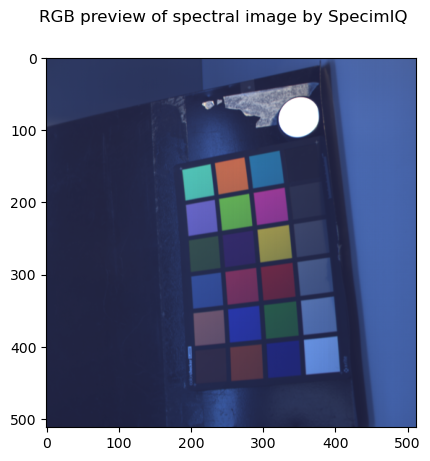
\includegraphics[width=0.45\textwidth]{fig-task1/specimIQ-rgb.png}
  }
  \caption[]{Previews of Specim IQ}
  \label{fig:specim-preview}
\end{figure}

\subsubsection{Plot pair of spectra in one}

\begin{figure}[H]
  \centering
  \caption{Plot pair of spectra in one}
  \label{fig:specim-plot}
  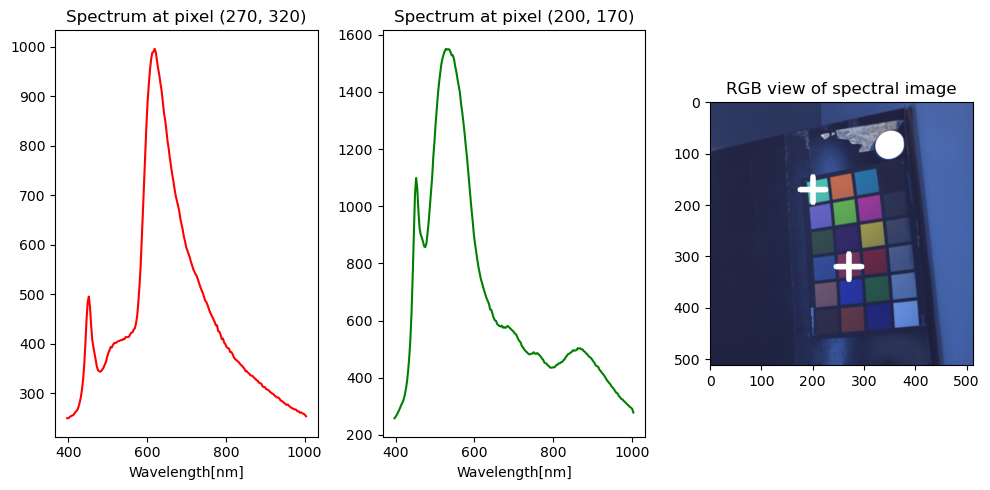
\includegraphics[width=0.8\textwidth]{fig-task1/specimIQ-plot.png}
\end{figure}

\subsection{Spectral Scanner}

Spectral image by Spectral Scanner was also processed by    the same Python script. The gray scale preview and RGB preview are shown in Figure \ref{fig:spectral-preview}.

The same codes, with diffrent path in Code \ref{code:show-gray-preview} and Code \ref{code:show-rgb-preview} were used to create the previews.

\subsubsection{Preview}

\begin{figure}[H] %
  \centering
  \subfloat[Gray scale preview]{%
    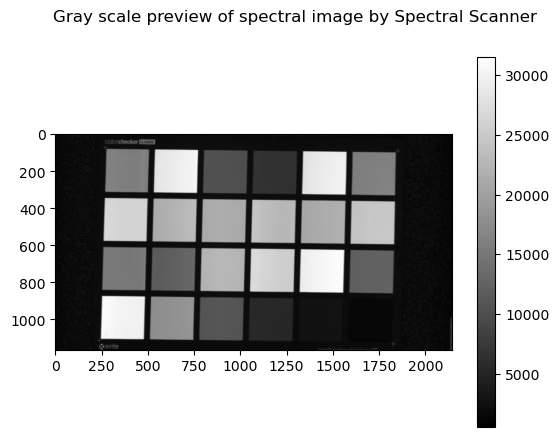
\includegraphics[width=0.45\textwidth]{fig-task1/spectral-scanner-gray.png}
  }
  \hspace{0.1cm}
  \subfloat[RGB preview]{%
    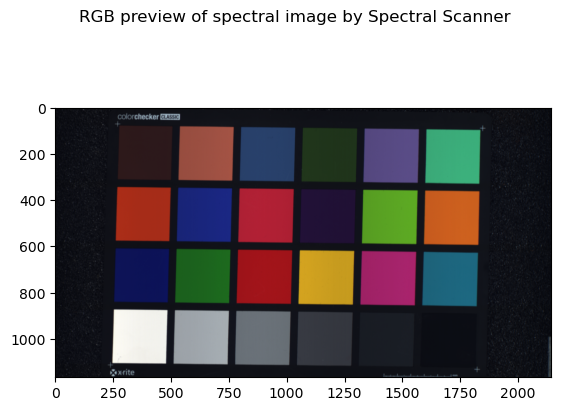
\includegraphics[width=0.45\textwidth]{fig-task1/spectral-scanner-rgb.png}
  }
  \caption[]{Previews of Spectral Scanner}
  \label{fig:spectral-preview}
\end{figure}

\subsubsection{Plot pair of spectra in one}

\begin{figure}[H]
  \centering
  \caption{Plot pair of spectra in one}
  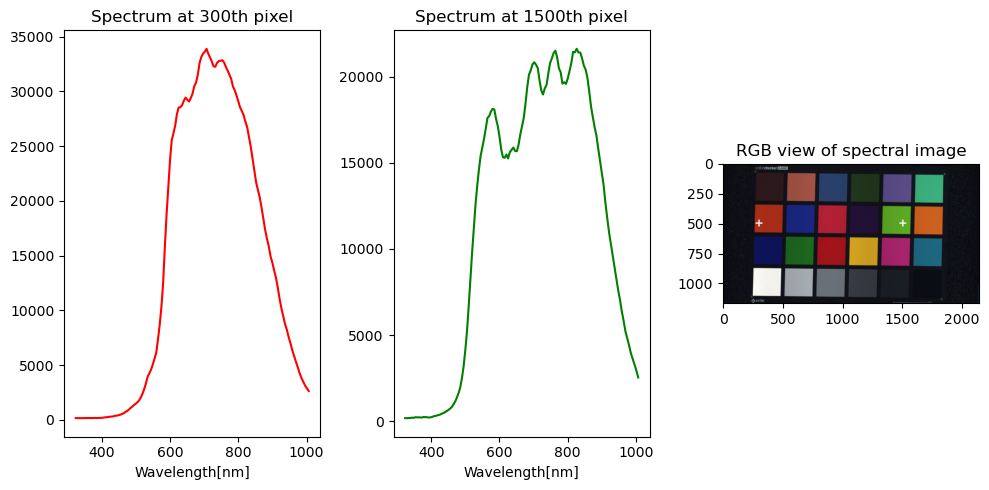
\includegraphics[width=0.8\textwidth]{fig-task1/spectral-scanner-plot.png}
  \label{fig:spectral-plot}
\end{figure}
